% Options for packages loaded elsewhere
\PassOptionsToPackage{unicode}{hyperref}
\PassOptionsToPackage{hyphens}{url}
%
\documentclass[
  ignorenonframetext,
]{beamer}
\usepackage{pgfpages}
\setbeamertemplate{caption}[numbered]
\setbeamertemplate{caption label separator}{: }
\setbeamercolor{caption name}{fg=normal text.fg}
\beamertemplatenavigationsymbolsempty
% Prevent slide breaks in the middle of a paragraph
\widowpenalties 1 10000
\raggedbottom
\setbeamertemplate{part page}{
  \centering
  \begin{beamercolorbox}[sep=16pt,center]{part title}
    \usebeamerfont{part title}\insertpart\par
  \end{beamercolorbox}
}
\setbeamertemplate{section page}{
  \centering
  \begin{beamercolorbox}[sep=12pt,center]{part title}
    \usebeamerfont{section title}\insertsection\par
  \end{beamercolorbox}
}
\setbeamertemplate{subsection page}{
  \centering
  \begin{beamercolorbox}[sep=8pt,center]{part title}
    \usebeamerfont{subsection title}\insertsubsection\par
  \end{beamercolorbox}
}
\AtBeginPart{
  \frame{\partpage}
}
\AtBeginSection{
  \ifbibliography
  \else
    \frame{\sectionpage}
  \fi
}
\AtBeginSubsection{
  \frame{\subsectionpage}
}
\usepackage{amsmath,amssymb}
\usepackage{lmodern}
\usepackage{iftex}
\ifPDFTeX
  \usepackage[T1]{fontenc}
  \usepackage[utf8]{inputenc}
  \usepackage{textcomp} % provide euro and other symbols
\else % if luatex or xetex
  \usepackage{unicode-math}
  \defaultfontfeatures{Scale=MatchLowercase}
  \defaultfontfeatures[\rmfamily]{Ligatures=TeX,Scale=1}
\fi
\usetheme[]{Frankfurt}
% Use upquote if available, for straight quotes in verbatim environments
\IfFileExists{upquote.sty}{\usepackage{upquote}}{}
\IfFileExists{microtype.sty}{% use microtype if available
  \usepackage[]{microtype}
  \UseMicrotypeSet[protrusion]{basicmath} % disable protrusion for tt fonts
}{}
\makeatletter
\@ifundefined{KOMAClassName}{% if non-KOMA class
  \IfFileExists{parskip.sty}{%
    \usepackage{parskip}
  }{% else
    \setlength{\parindent}{0pt}
    \setlength{\parskip}{6pt plus 2pt minus 1pt}}
}{% if KOMA class
  \KOMAoptions{parskip=half}}
\makeatother
\usepackage{xcolor}
\IfFileExists{xurl.sty}{\usepackage{xurl}}{} % add URL line breaks if available
\IfFileExists{bookmark.sty}{\usepackage{bookmark}}{\usepackage{hyperref}}
\hypersetup{
  pdftitle={V and R},
  pdfauthor={Edwin de Jonge},
  hidelinks,
  pdfcreator={LaTeX via pandoc}}
\urlstyle{same} % disable monospaced font for URLs
\newif\ifbibliography
\usepackage{color}
\usepackage{fancyvrb}
\newcommand{\VerbBar}{|}
\newcommand{\VERB}{\Verb[commandchars=\\\{\}]}
\DefineVerbatimEnvironment{Highlighting}{Verbatim}{commandchars=\\\{\}}
% Add ',fontsize=\small' for more characters per line
\usepackage{framed}
\definecolor{shadecolor}{RGB}{248,248,248}
\newenvironment{Shaded}{\begin{snugshade}}{\end{snugshade}}
\newcommand{\AlertTok}[1]{\textcolor[rgb]{0.94,0.16,0.16}{#1}}
\newcommand{\AnnotationTok}[1]{\textcolor[rgb]{0.56,0.35,0.01}{\textbf{\textit{#1}}}}
\newcommand{\AttributeTok}[1]{\textcolor[rgb]{0.77,0.63,0.00}{#1}}
\newcommand{\BaseNTok}[1]{\textcolor[rgb]{0.00,0.00,0.81}{#1}}
\newcommand{\BuiltInTok}[1]{#1}
\newcommand{\CharTok}[1]{\textcolor[rgb]{0.31,0.60,0.02}{#1}}
\newcommand{\CommentTok}[1]{\textcolor[rgb]{0.56,0.35,0.01}{\textit{#1}}}
\newcommand{\CommentVarTok}[1]{\textcolor[rgb]{0.56,0.35,0.01}{\textbf{\textit{#1}}}}
\newcommand{\ConstantTok}[1]{\textcolor[rgb]{0.00,0.00,0.00}{#1}}
\newcommand{\ControlFlowTok}[1]{\textcolor[rgb]{0.13,0.29,0.53}{\textbf{#1}}}
\newcommand{\DataTypeTok}[1]{\textcolor[rgb]{0.13,0.29,0.53}{#1}}
\newcommand{\DecValTok}[1]{\textcolor[rgb]{0.00,0.00,0.81}{#1}}
\newcommand{\DocumentationTok}[1]{\textcolor[rgb]{0.56,0.35,0.01}{\textbf{\textit{#1}}}}
\newcommand{\ErrorTok}[1]{\textcolor[rgb]{0.64,0.00,0.00}{\textbf{#1}}}
\newcommand{\ExtensionTok}[1]{#1}
\newcommand{\FloatTok}[1]{\textcolor[rgb]{0.00,0.00,0.81}{#1}}
\newcommand{\FunctionTok}[1]{\textcolor[rgb]{0.00,0.00,0.00}{#1}}
\newcommand{\ImportTok}[1]{#1}
\newcommand{\InformationTok}[1]{\textcolor[rgb]{0.56,0.35,0.01}{\textbf{\textit{#1}}}}
\newcommand{\KeywordTok}[1]{\textcolor[rgb]{0.13,0.29,0.53}{\textbf{#1}}}
\newcommand{\NormalTok}[1]{#1}
\newcommand{\OperatorTok}[1]{\textcolor[rgb]{0.81,0.36,0.00}{\textbf{#1}}}
\newcommand{\OtherTok}[1]{\textcolor[rgb]{0.56,0.35,0.01}{#1}}
\newcommand{\PreprocessorTok}[1]{\textcolor[rgb]{0.56,0.35,0.01}{\textit{#1}}}
\newcommand{\RegionMarkerTok}[1]{#1}
\newcommand{\SpecialCharTok}[1]{\textcolor[rgb]{0.00,0.00,0.00}{#1}}
\newcommand{\SpecialStringTok}[1]{\textcolor[rgb]{0.31,0.60,0.02}{#1}}
\newcommand{\StringTok}[1]{\textcolor[rgb]{0.31,0.60,0.02}{#1}}
\newcommand{\VariableTok}[1]{\textcolor[rgb]{0.00,0.00,0.00}{#1}}
\newcommand{\VerbatimStringTok}[1]{\textcolor[rgb]{0.31,0.60,0.02}{#1}}
\newcommand{\WarningTok}[1]{\textcolor[rgb]{0.56,0.35,0.01}{\textbf{\textit{#1}}}}
\setlength{\emergencystretch}{3em} % prevent overfull lines
\providecommand{\tightlist}{%
  \setlength{\itemsep}{0pt}\setlength{\parskip}{0pt}}
\setcounter{secnumdepth}{-\maxdimen} % remove section numbering

\ifLuaTeX
  \usepackage{selnolig}  % disable illegal ligatures
\fi

\title{V and R}
\subtitle{rvee: recreational v programming for R}
\author{Edwin de Jonge}
\date{Statistics Netherlands / UseR! 2022, @edwindjonge}

\begin{document}
\frame{\titlepage}

\begin{frame}[plain,fragile]{}
\protect\hypertarget{section}{}
\begin{centering}
  
\includegraphics[width=0.8\paperwidth]{img/rv}
  \par
\end{centering}
\end{frame}

\begin{frame}[fragile]{Who am I?}
\protect\hypertarget{who-am-i}{}
\begin{block}{Edwin de Jonge}
\protect\hypertarget{edwin-de-jonge}{}
\begin{itemize}
\tightlist
\item
  Statistical Consultant / R\&D at Statistics Netherlands / CBS
\item
  Author of some R packages (e.g.~\texttt{whisker}, \texttt{docopt}):
  \url{https://edwindj.r-universe.dev}
\item
  Love R and like programming in general
\item
  \url{http://github.com/edwindj}, @edwindjonge
\end{itemize}
\end{block}
\end{frame}

\begin{frame}[fragile]{Short summary}
\protect\hypertarget{short-summary}{}
\large

\begin{itemize}
\item
  \texttt{V} new simple programming language
\item
  \texttt{rvee} : \url{https://github.com/edwindj/rvee} helps to create
  R extension in V.
\item
  No runtime and R dependencies.
\item
  Experimental, but works.
\end{itemize}
\end{frame}

\begin{frame}[fragile]{What is V?}
\protect\hypertarget{what-is-v}{}
\begin{itemize}
\tightlist
\item
  V is a programming language.
\end{itemize}

\begin{quote}
Simple.fase, safe, compiled. For developing maintainable software.
\end{quote}

\begin{itemize}
\tightlist
\item
  Website: \url{https://vlang.io/}
\item
  young, low-level,
\item
  feels like scripting, but is strongly typed
\item
  Very similar to \texttt{Go}, but ``improves'' on Go:
  \url{https://vlang.io/compare\#go}
\item
  Very light weight
\end{itemize}
\end{frame}

\begin{frame}{\{.plain .fragile\} Syntax example}
\protect\hypertarget{plain-.fragile-syntax-example}{}
\begin{centering}
  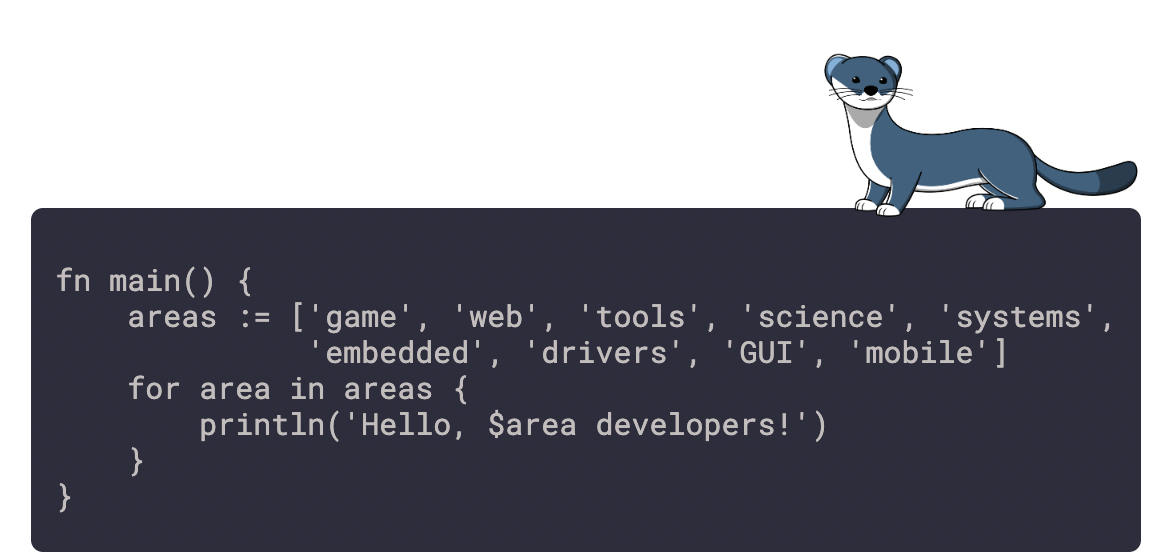
\includegraphics[width=0.8\paperwidth]{img/example.v}
  \par
\end{centering}
\end{frame}

\begin{frame}[fragile]{V is safe}
\protect\hypertarget{v-is-safe}{}

\includegraphics[width=0.1\paperwidth]{img/vlang}

\begin{itemize}
\tightlist
\item
  No \texttt{null}, \texttt{undefined} values: unexpected \texttt{null}
  causes software damage.
\item
  \textbf{immutable} variables by default, making it easier to optimize
  and reason about code
\item
  \textbf{Option}: functions returns \texttt{?Type} and compiler
  generates error is empty return is not handled properly.
\item
  \textbf{Result}: functions can return \texttt{!Type} and compiler
  generates error if run-time error is not handled properly.
\item
  Other cases a function always returns a value
\item
  Functions are pure by default (impurity is explicit)
\end{itemize}
\end{frame}

\begin{frame}{V features}
\protect\hypertarget{v-features}{}
\begin{itemize}
\tightlist
\item
  Easy C-interop (C-backend)
\item
  Fast compilation!
\item
  Zero cost abstractions
\item
  Sum Types
\item
  Generics
\end{itemize}
\end{frame}

\begin{frame}[plain,fragile]{Fast compilation}
\protect\hypertarget{fast-compilation}{}
\begin{centering}
  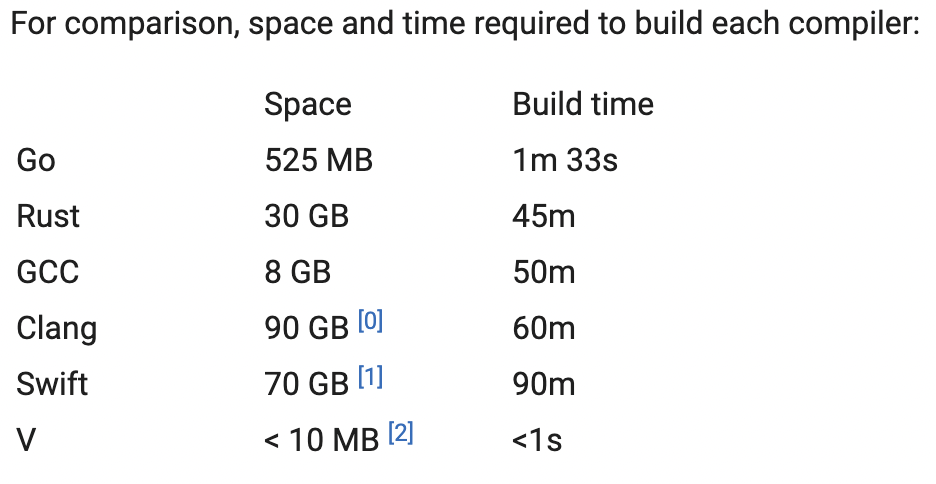
\includegraphics[width=0.8\paperwidth]{img/compilation}
  \par
\end{centering}

\tiny source: \url{https://vlang.io}
\end{frame}

\begin{frame}[fragile]{Performance (from V lang website)}
\protect\hypertarget{performance-from-v-lang-website}{}
\begin{itemize}
\tightlist
\item
  As fast as C (V's main backend compiles to human readable C)
\item
  C interop without any costs
\item
  Minimal amount of allocations
\item
  Built-in serialization without runtime reflection
\item
  Compiles to native binaries without any dependencies: a simple web
  server is only 65 KB
\end{itemize}

\begin{block}{V has different compilation back-ends (like rust and Go)}
\protect\hypertarget{v-has-different-compilation-back-ends-like-rust-and-go}{}
\begin{itemize}
\tightlist
\item
  native code (includes a REPL)
\item
  readable(!) \texttt{C} code
\item
  javascript
\end{itemize}
\end{block}
\end{frame}

\begin{frame}[fragile]{R similarities}
\protect\hypertarget{r-similarities}{}
\begin{itemize}
\tightlist
\item
  V functions are \emph{pure} by default, like R, arguments are
  immutable by default. Have to be marked \texttt{mut}able.
\item
  V has \texttt{defer}, like R's \texttt{on.exit}
\item
  Simple syntax, very flexible
\item
  Has (some) reflection/code generation. (R beats that one)
\end{itemize}
\end{frame}

\begin{frame}[fragile]{V pkgs}
\protect\hypertarget{v-pkgs}{}
\begin{itemize}
\tightlist
\item
  V has a module and pkg system, containing \texttt{v} src code (not
  compiled)
\item
  Typical v-compilation results in one binary
\item
  importing a module means including the v code.
\item
  v can link though to \texttt{C}, \texttt{CPP} libraries.
\end{itemize}
\end{frame}

\begin{frame}[fragile]{What is \texttt{rvee}?}
\protect\hypertarget{what-is-rvee}{}
\begin{itemize}
\tightlist
\item
  An experimental R package to create R package extensions with
  functions written in V.
\item
  Similar in concept to RCpp but for V.
\item
  But no \emph{compile-time} and \emph{run-time} dependencies in
  resulting R package.
\item
  (pkgname \texttt{rv} was already claimed for)
\end{itemize}

\begin{block}{Why-o-why}
\protect\hypertarget{why-o-why}{}
\begin{itemize}
\tightlist
\item
  One of R's great powers is that of a glue language (just like S)
\item
  V is a nice low-level language, so why not?
\item
  Because it is fun :-)
\end{itemize}
\end{block}
\end{frame}

\begin{frame}[fragile]{Features \texttt{rvee}}
\protect\hypertarget{features-rvee}{}
Two possible routes for using \texttt{v} as extension for R: - Use v
compiler to link to \texttt{R.so} / \texttt{R.dll}, but requires v to be
present on CRAN. - Use v transpiler to C and create a ``normal'' R
package. This is \texttt{rvee}

\begin{block}{\texttt{rvee}}
\protect\hypertarget{rvee}{}
\begin{itemize}
\tightlist
\item
  Transpiles v code into C package code, including all wrappers
\item
  include \texttt{vpkg}:\texttt{r} with wrapper functions for R's C API
  (30\% complete, vector stuff works)
\end{itemize}
\end{block}
\end{frame}

\begin{frame}[fragile]{\texttt{rvee::rv\_export\_c}}
\protect\hypertarget{rveerv_export_c}{}
\begin{itemize}
\item
  Put the v source in \texttt{"\textless{}pkg\textgreater{}/src/v"}
  directory
\item
  decorate each function to be exported with \texttt{{[}rv\_export{]}}
  attribute
\item
  \texttt{rvee::rv\_export\_c("\textless{}pkg\textgreater{}")}
  generates:

  \begin{itemize}
  \tightlist
  \item
    ``./R/rv\_export.R'': R functions calling the v functions declared
    in ``./src/v/rv\_export.v''
  \item
    ``./src/v/rv\_export.v'': v wrapper functions translating input and
    output to the original v functions.
  \item
    ``./src/init.c'': registration code for the shared library
  \item
    ``./src/.c'': the c code generated by v from the source files in the
    ``/src/v'' directory.
  \end{itemize}
\item
  And ready! No dependencies what so ever.
\item
  After that \texttt{devtools::load\_all} (or \texttt{R\ CMD\ SHLIB})
  work. (on the generated C files)
\end{itemize}
\end{frame}

\begin{frame}[fragile]{Other \texttt{v\_function}}
\protect\hypertarget{other-v_function}{}
\begin{itemize}
\tightlist
\item
  \texttt{v\_function} generates from v src code a working R function
  that calls that code
\end{itemize}

\begin{Shaded}
\begin{Highlighting}[]
\FunctionTok{v\_function}\NormalTok{(}\StringTok{\textquotesingle{}fn add(x int, y int, z int) int\{}
\StringTok{  sum := x + y + z}
\StringTok{  return sum}
\StringTok{\}\textquotesingle{}}\NormalTok{)}

\FunctionTok{add}\NormalTok{(}\DecValTok{1}\NormalTok{,}\DecValTok{2}\NormalTok{,}\DecValTok{3}\NormalTok{)}
\end{Highlighting}
\end{Shaded}

\begin{block}{vpkg \texttt{r}}
\protect\hypertarget{vpkg-r}{}
\begin{itemize}
\tightlist
\item
  wrapper library for R API.
\item
  helps to transform V strings, arrays into R vectors (and vice versa).
\end{itemize}
\end{block}
\end{frame}

\begin{frame}{Status \texttt{rvee}}
\protect\hypertarget{status-rvee}{}
\begin{itemize}
\tightlist
\item
  V is a young language, but already quite stable.
\item
  Generated code is in C
\item
  rvee is experimental,
\item
  Help is welcome!
\item
  Experimental, expect (breaking) changes!
\item
  But\ldots, hey it works :-)
\end{itemize}
\end{frame}

\begin{frame}[fragile]{Thank you!}
\protect\hypertarget{thank-you}{}
\Large Interested?

\begin{Shaded}
\begin{Highlighting}[]
\NormalTok{remotes}\SpecialCharTok{::}\FunctionTok{install\_github}\NormalTok{(}\StringTok{"edwindj/rvee"}\NormalTok{)}
\end{Highlighting}
\end{Shaded}

Or visit:

\href{http://github.com/edwindj/rvee}{\textbf{http://github.com/edwindj/rvee}}
\end{frame}

\end{document}
